\documentclass[12pt]{report}
\usepackage[margin=1in]{geometry}
\usepackage{xcolor}
\usepackage{fontspec}
\usepackage{graphicx}
\usepackage{tabularx}
\usepackage{authoraftertitle}
\usepackage{xltabular}

\title{Criterion B: Design}
\definecolor{msblue}{HTML}{5AB5D8}
\makeatletter
\graphicspath{{images/}}
\newenvironment{code}{\ttfamily}{\par}

\begin{document}
\centerline{\textcolor{msblue}{
    \fontspec{Cambria}\textbf{\fontsize{13}{13}\MyTitle}
  }}

\section*{UML Diagram}
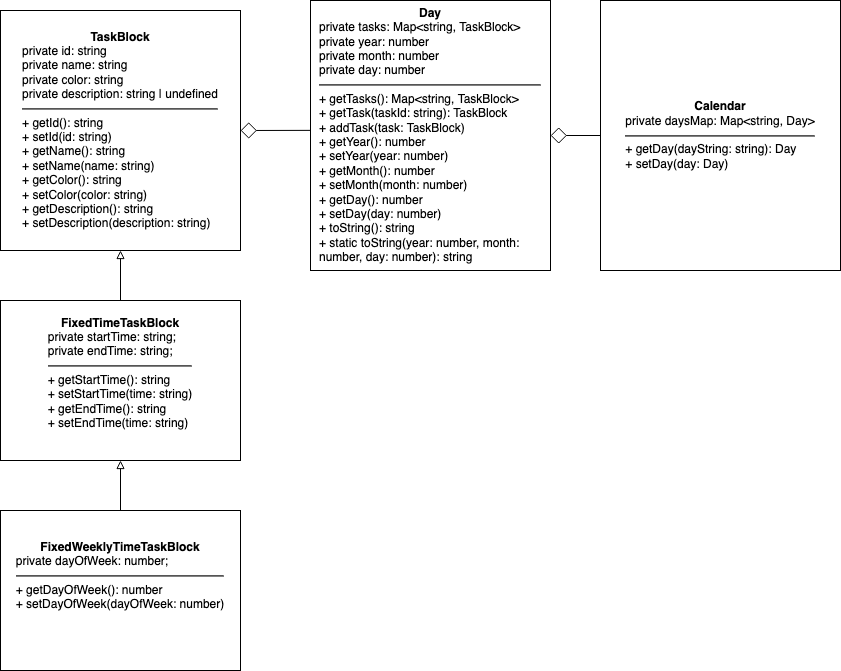
\includegraphics[width=\textwidth]{uml-diagram.png}

\section*{Flowchart}
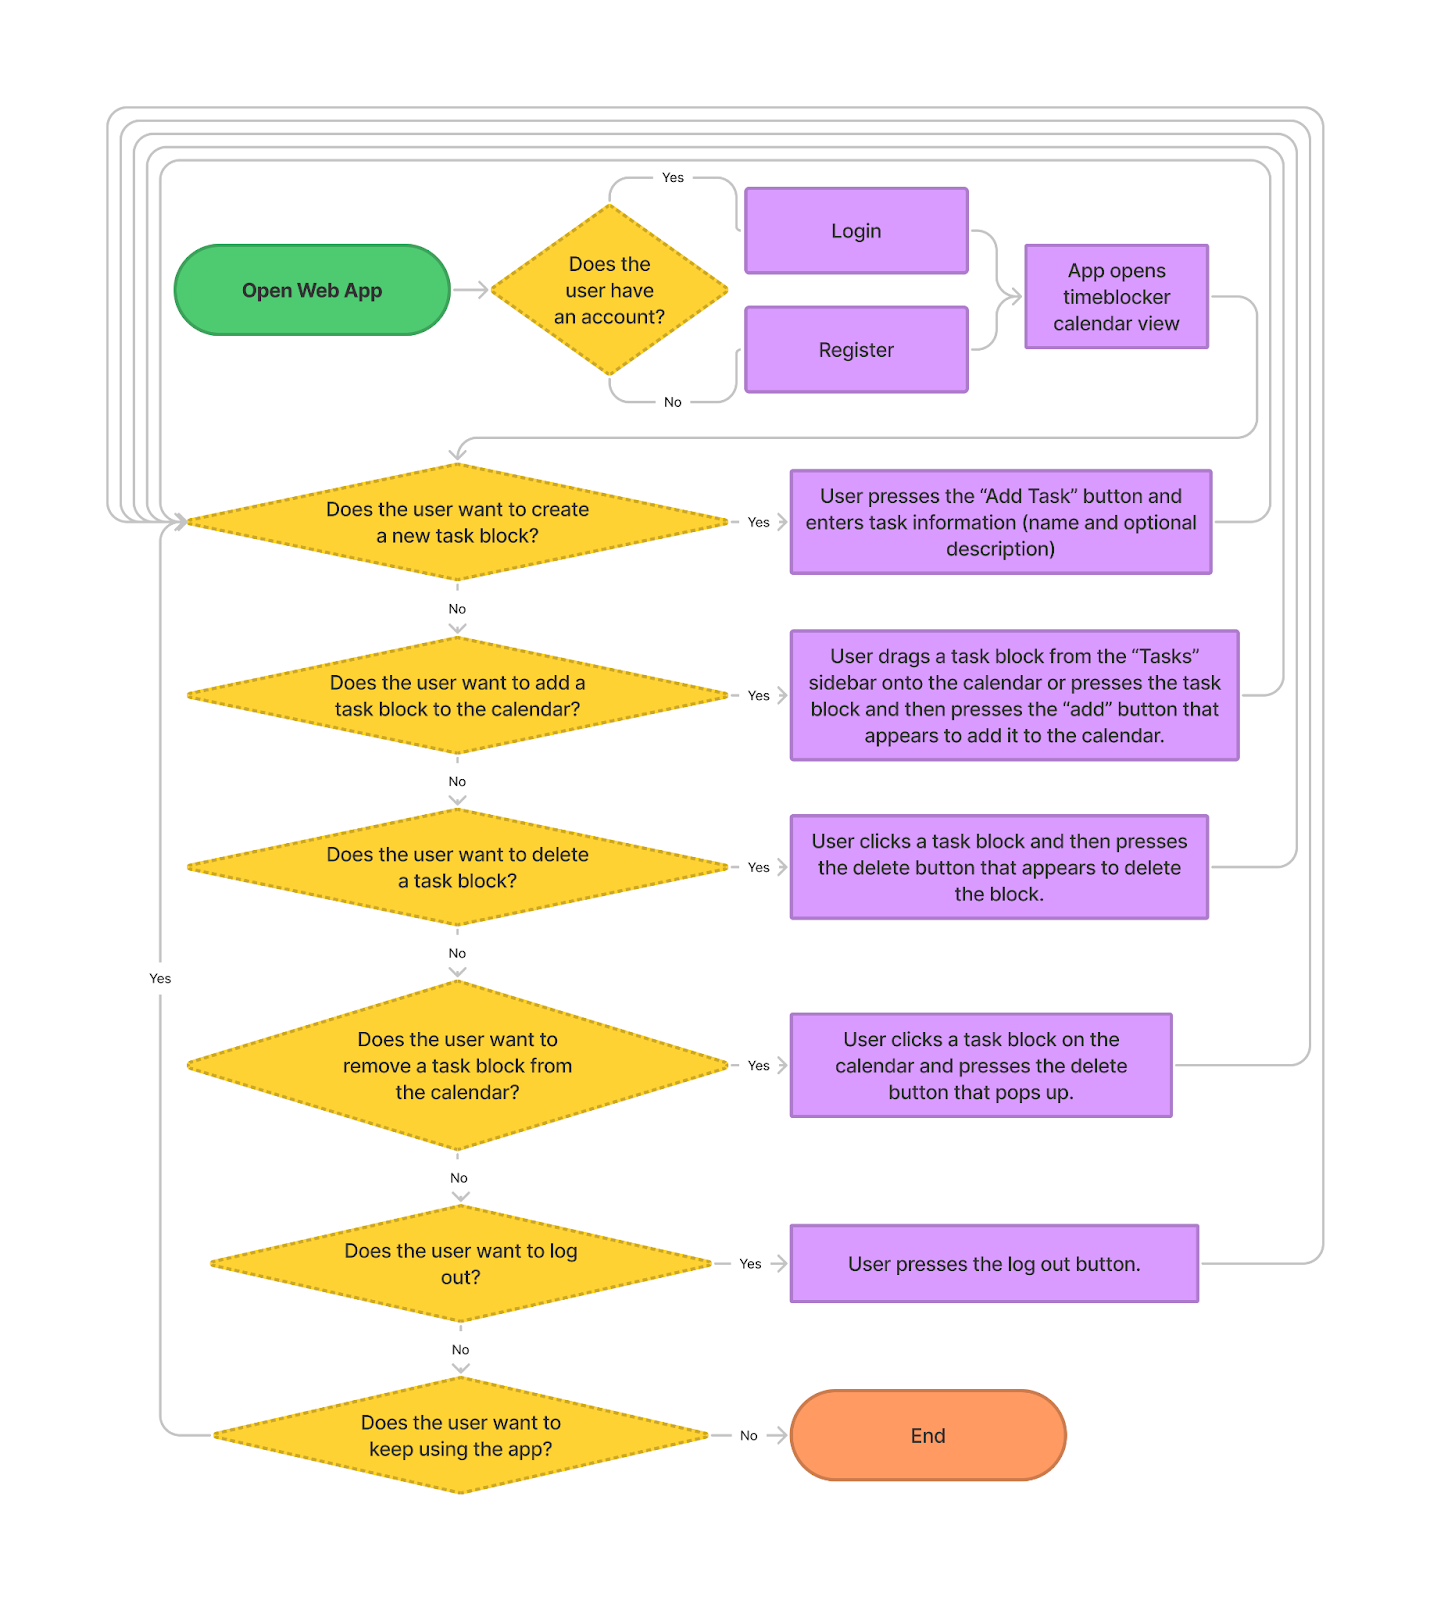
\includegraphics[width=\textwidth]{flowchart.png}

\section*{UI Design}
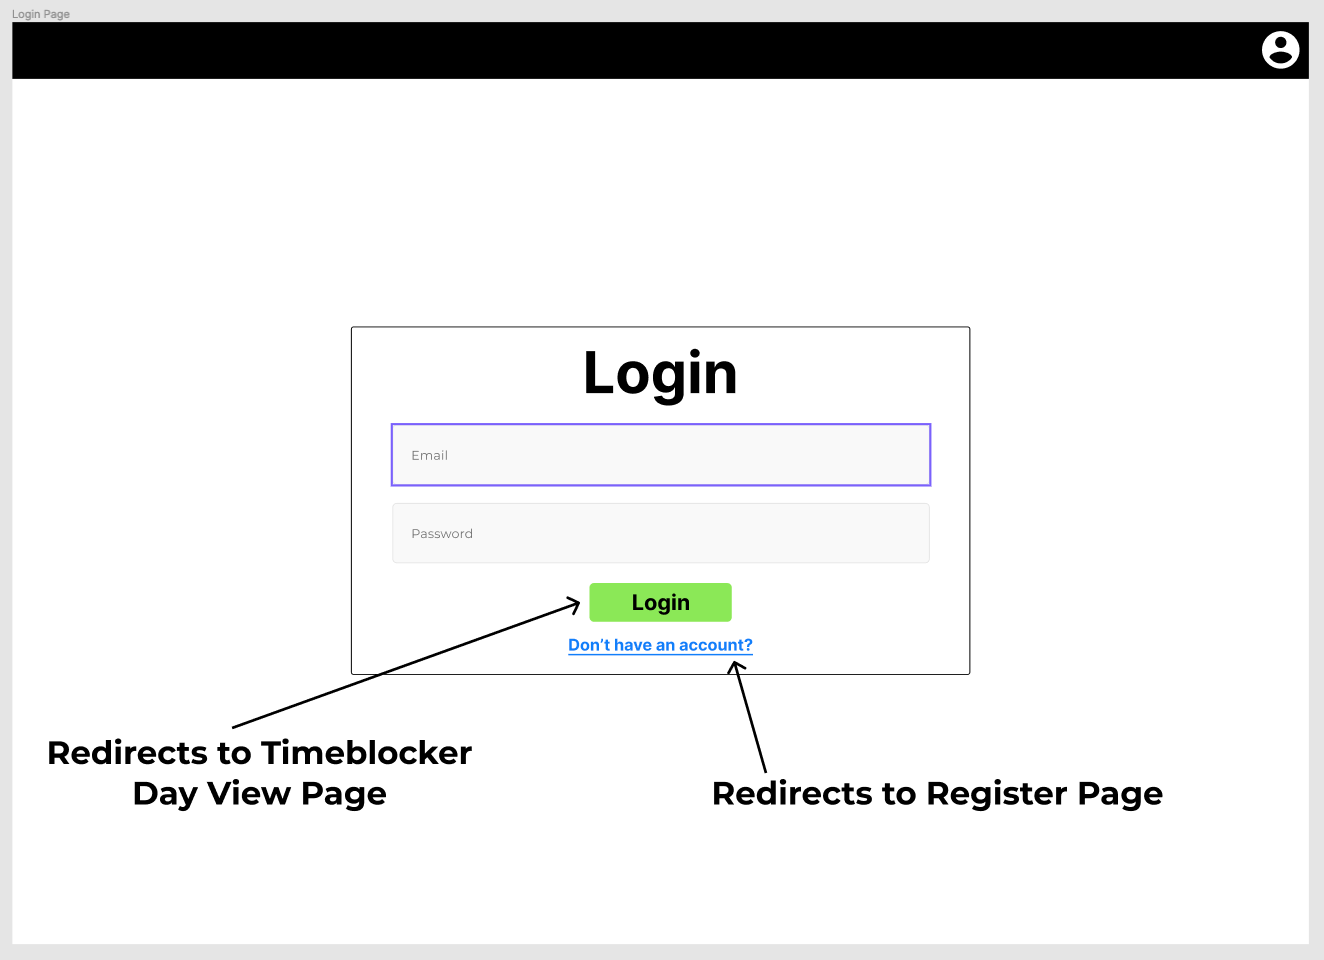
\includegraphics[width=\textwidth]{login-page.png}
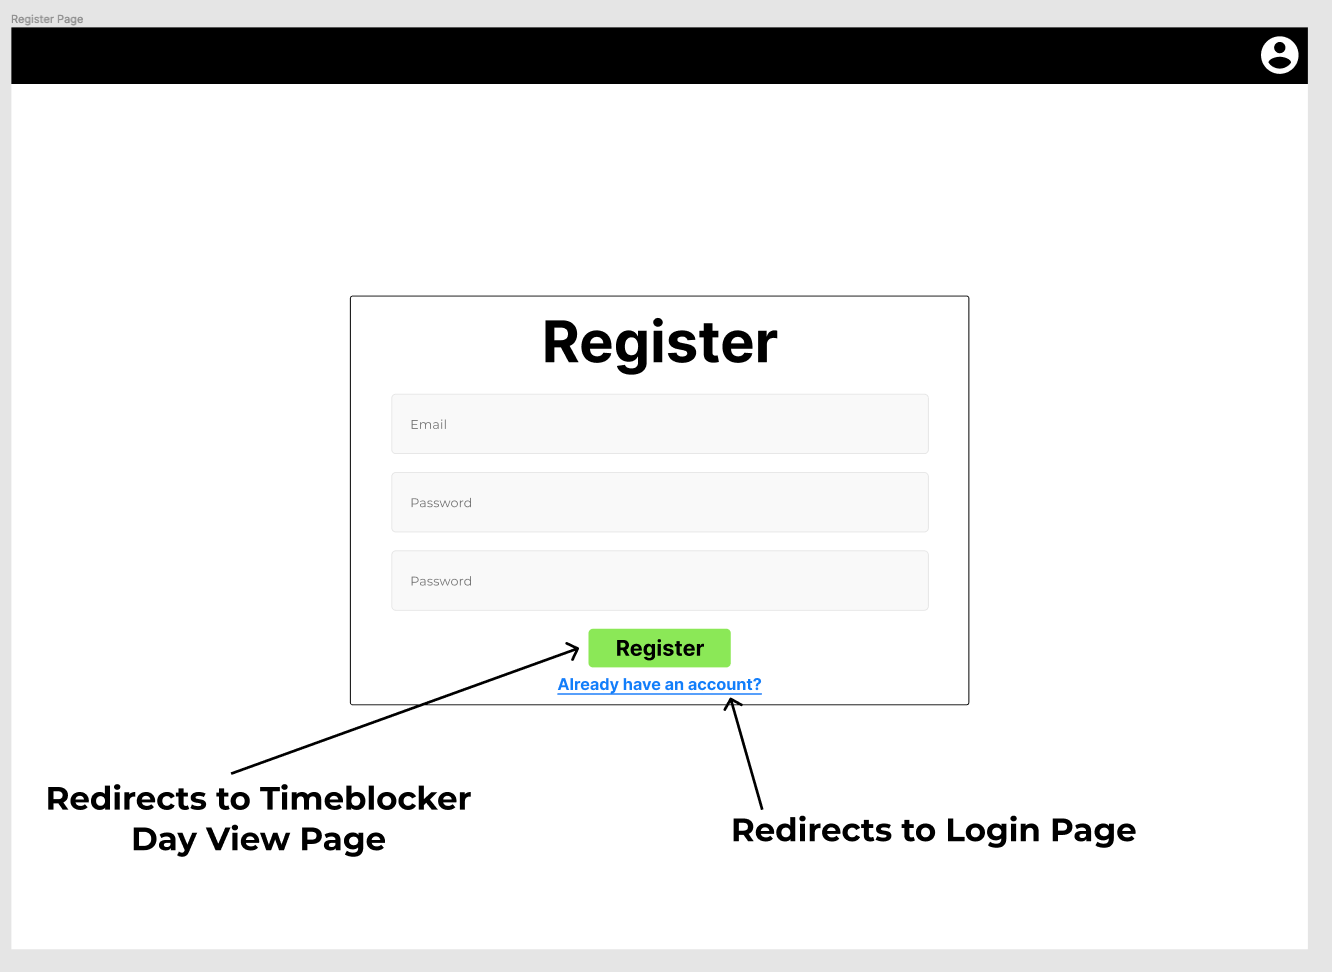
\includegraphics[width=\textwidth]{register-page.png}
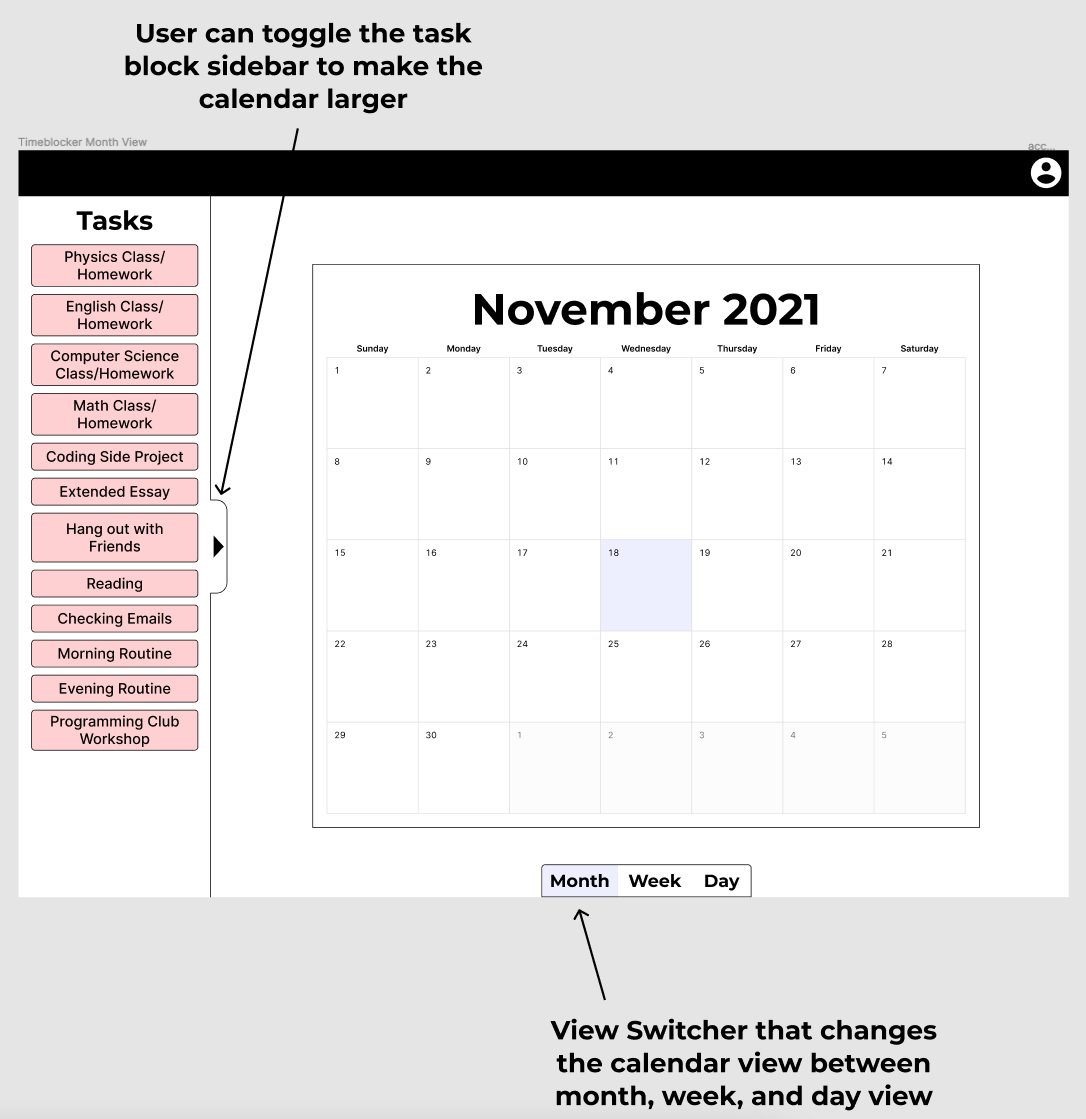
\includegraphics[width=\textwidth]{month-view.png}
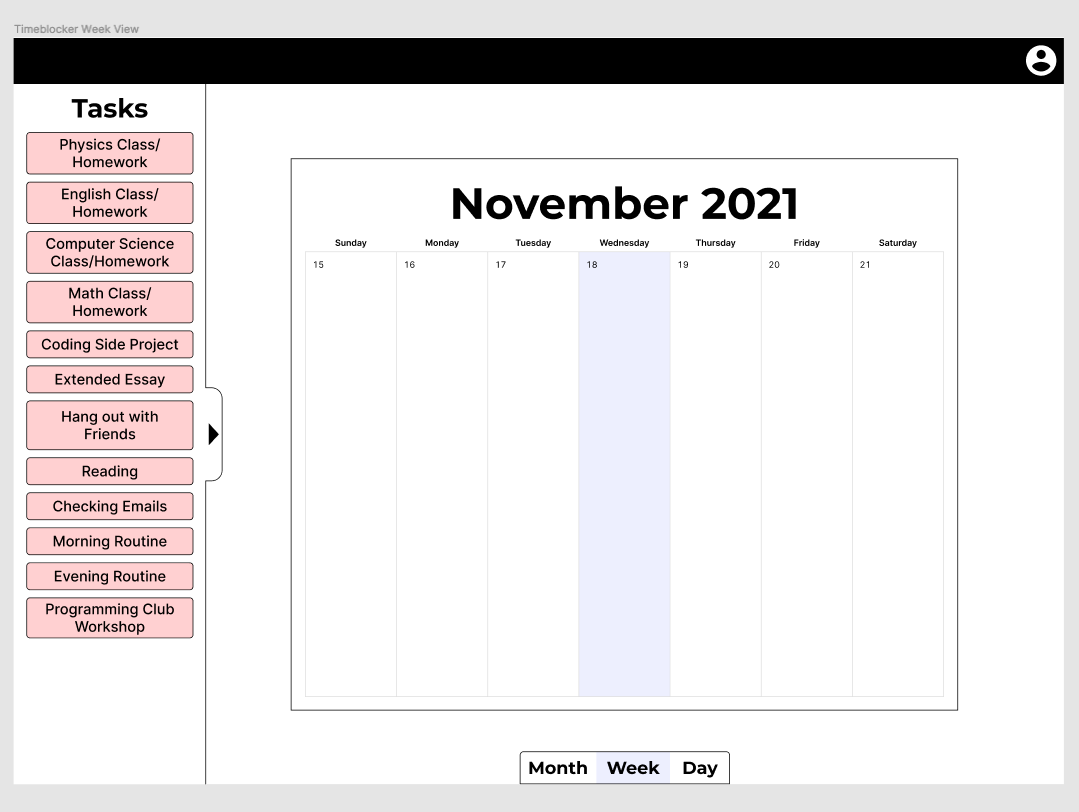
\includegraphics[width=\textwidth]{week-view.png}
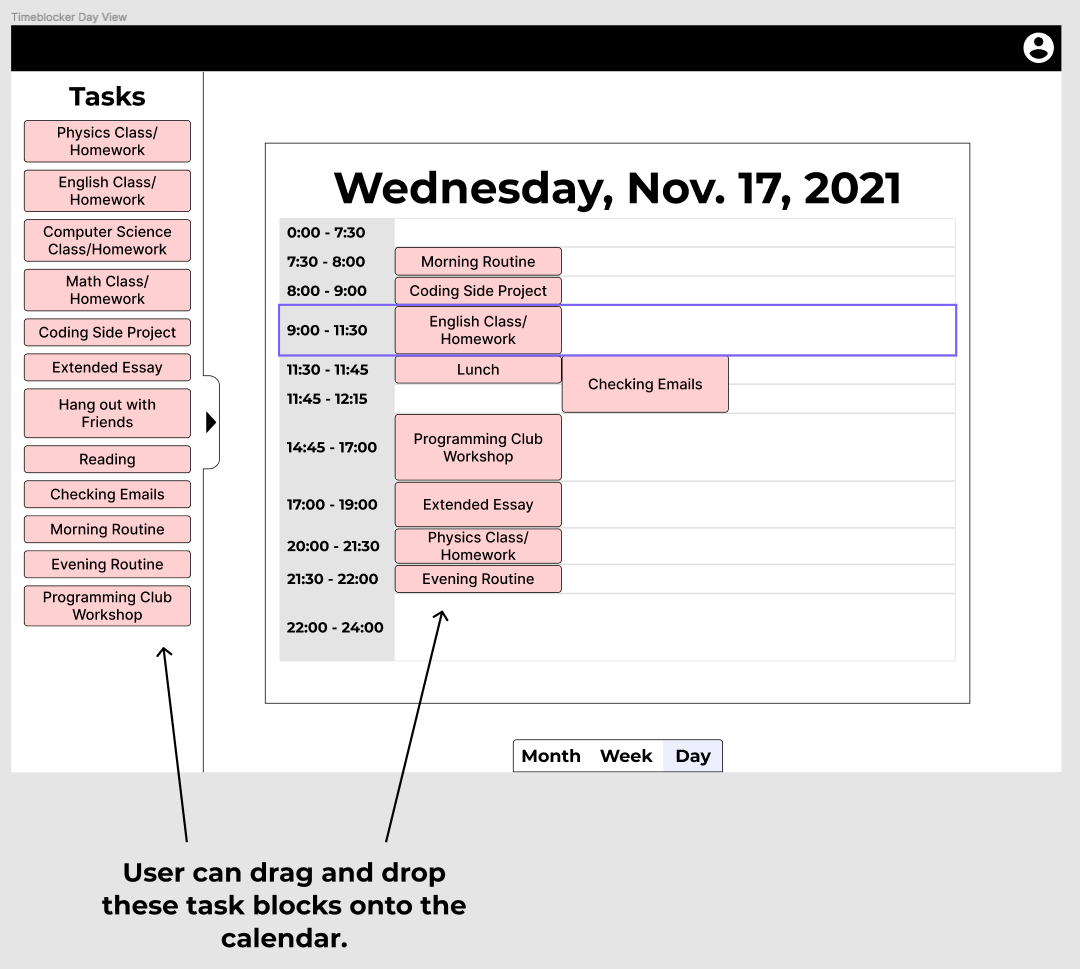
\includegraphics[width=\textwidth]{day-view.png}

\newpage

\section*{Algorithms}

\subsection*{Merge Sort}
\begin{verbatim}
// The comparison function returns true if the first element is less than the second element
function merge (leftArray, rightArray, comparisonFunction)
  sortedArray = []
  leftIndex = 0
  rightIndex = 0

  while leftIndex < leftArray.length and rightIndex < rightArray.length
    // If the left element is less than the right element
    if comparisonFunction(left[leftIndex], right[rightIndex])
      sortedArray.push(left[leftIndex])
      leftIndex += 1
    else
      sortedArray.push(right[rightIndex])
      rightIndex += 1

  return sortedArray +
    remaining elements of left array +
    remaining elements of right array

function mergeSort (array, comparisonFunction)
  half = array.length / 2

  if array.length < 2
    return array

  left = array.slice(0, half)
  right = array.slice(half, array.length)

  return merge(
    mergeSort(left, comparisonFunction),
    mergeSort(right, comparisonFunction)
  )
\end{verbatim}

\newpage
\section*{Product Development Plan}
\def\arraystretch{1.5}
\begin{xltabular}{\textwidth}{|X|X|}
  \hline
  Function
   & Comments
  \\\hline
  Landing Page

  \medskip

  \textbf{Time:} 1 week
  &
  The landing page should contain a description of the app's features, as well as a call to action and the Login and Register buttons that allow the user to easily create a new account.
  \\\hline
  Account Entry Screens
  \begin{itemize}
    \item Login Screen
    \item Register Screen
  \end{itemize}
  \textbf{Time:} 3 weeks
   &
  To synchronize the user's calendar across multiple devices, they’ll need to create and log into a Timeblocker account. I need to store their information security using standard web security practices such as password hashing.
  \\\hline
  The Task Blocks Sidebar
  \begin{itemize}
    \item Ability to create, edit, and delete task blocks
    \item Sorting and searching functions.
    \item Creating different types of task blocks
  \end{itemize}
  \textbf{Time:} 3 weeks
   &
  The user needs to be able to manage their task blocks on the sidebar, with the ability to add different types of tasks and sort the tasks based on the name.
  \\\hline
  The Calendar View
  \begin{itemize}
    \item Able to see a calendar and create a timeblock for any day on the calendar.
    \item Ability to see a time-based (hour-by-hour) view when viewing a timeblock schedule for a specific day.
  \end{itemize}
  \textbf{Time:} 2 weeks
   &
  The calendar should allow the user to navigate between various months and see all the days where they've already created a timeblock. When viewing a timeblock for a specific day, the user must be able to interact with the timeblock schedule and have the ability to drag nd resize tasks to reorder them.
  \\\hline
\end{xltabular}

\end{document}